\documentclass[a4paper]{article}
\usepackage[french]{babel}
\usepackage{geometry}
\geometry{a4paper}
\usepackage[utf8]{inputenc}
\usepackage{graphicx}
\graphicspath{ {./image/} }
\usepackage{amsmath}
\usepackage{amssymb}
\usepackage{listings}
\usepackage{xcolor}
\usepackage{cite}
\usepackage{color}
\usepackage{float}
\usepackage{soul}


\definecolor{mGreen}{rgb}{0,0.6,0}
\definecolor{mGray}{rgb}{0.5,0.5,0.5}
\definecolor{mPurple}{rgb}{0.58,0,0.82}
\definecolor{backgroundColour}{rgb}{0.95,0.95,0.92}

\lstdefinestyle{CStyle}{
    backgroundcolor=\color{backgroundColour},   
    commentstyle=\color{mGreen},
    keywordstyle=\color{magenta},
    numberstyle=\tiny\color{mGray},
    stringstyle=\color{mPurple},
    basicstyle=\footnotesize,
    breakatwhitespace=false,         
    breaklines=true,                 
    captionpos=b,                    
    keepspaces=true,                 
    numbers=left,                    
    numbersep=5pt,                  
    showspaces=false,                
    showstringspaces=false,
    showtabs=false,                  
    tabsize=2,
    language=C
}          

\title{\textbf{projet} \\ document}

\author{Louison GOUY \and Yiying WEI}

\begin{document}
\maketitle

\vspace{2cm}

\begin{center}
   % \includegraphics[width=12cm]{logo_tp.jpg}
\end{center}

\vspace*{1cm}

\begin{center}
    name
\end{center}

\vspace*{7cm}

\begin{center}

abstract
\end{center}

\newpage
\vspace*{3cm}
\begin{quotation}
	It's not you can use C to generate good code for hardware. If you think like a comupter writing C actually makes sens.
\end{quotation}
\begin{flushright}
	Linus Torvalds
\end{flushright} 
\newpage


\newpage
\renewcommand{\contentsname}{Table des Matières}
\tableofcontents
\newpage
\renewcommand\listfigurename{Liste des figures}
\listoffigures
\newpage
\section{Le langage C}
Le langage C est un langage combiné, il a les caractéristiques des langages évolués (boucles itératives etc.) associé à des fonctionnalités des langages assemblés (décalage de bit, adressage indirect généralisé etc.). C'est la combinaison de ces deux caractéristiques qui font la force du langage\cite{Monteil2012}. Sa proximité avec l'assembleur le rendant très efficace, il est ainsi devenu le langage indispensable dans la programmation des applications comme l'automatique, la robotique, les OS ect. Cette même proximité impose peu de contraintes à l'utilisateur sur la structure de son programme. Aussi, il est possible d'écrire des fonctions avec plusieurs points de sorties, ou encore, d'échapper à une boucle avant son terme. Là où certains trouveront une grande souplesse, les critiques le considérerons trop permissive. On notera qu'un certain nombre d'organismes officiels proposent un ensemble de règles visant, tout en conservant son efficacité, à éviter les problèmes liés à une programmation peu soignée. L'Agence National de la Sécurité des Systèmes Informatiques française (ANSSI) propose un rapport complet, \textit{Règles de programmation pour le développement sécurisé de logiciels en langage C}\cite{ANSSI2021}, visant à "favoriser la production de logiciels C plus sécurisés, plus sûrs, d’une plus grande robustesse et portables". Il servira de référence durant ce projet.

\newpage

\section{Programme de base} % touver un meilleur titre

Dans un premier temps un nouveau projet est créé de type "GCC C ASF Board project". Microchip studio génère alors une arborescence de fichiers dont un main.c. Ce dernier est étudié de manière globale puis affinée par étape dans la section suivante.

\subsection{Vue globale}
Cette partie détaille le fonctionnement du programme de base. 


\begin{lstlisting}[style=CStyle]
#include <asf.h>

int main (void)
{
	system_init();
	
	/* Insert application code here, after the board has been initialized. */
	
	/* This skeleton code simply sets the LED to the state of the button. */
	while (1) {
		/* Is button pressed? */
		if (port_pin_get_input_level(BUTTON_0_PIN) == BUTTON_0_ACTIVE) {
			/* Yes, so turn LED on. */
			port_pin_set_output_level(LED_0_PIN, LED_0_ACTIVE);
		} else {
			/* No, so turn LED off. */
			port_pin_set_output_level(LED_0_PIN, !LED_0_ACTIVE);
		}
	}
}
\end{lstlisting}
La première ligne permet d'inclure la  bibliothèque asf et ainsi de profiter du niveau d'abstraction mis à disposition par Microship. La suivante, \texttt{int main ()} bien connue des développeurs C, est le point d'entré du programme. C'est la première fonction exécutée. La ligne 5 \texttt{system\_init();} a été générée automatiquement par le logiciel à la création du projet. C'est elle qui nous offre ce niveau d'abstraction en initialisant les horloges et les entrées/sorties etc. Elle est spécifique à la cible utilisée, dans notre cas la carte Microchip SAMD21 Xplained Pro. La ligne 10 correspond à l'implémentation d'une boucle infinie. Cette dernière permet de lire l'état du bouton (ligne 12) en "continu". La condition suivante d’éclanche le résultat souhaité : allumage ou extinction de la LED0.

\subsection{Affinage}

\paragraph{Include ASF}
~~\\
L'Advanced Software Framework (ASF) fournit un riche ensemble de pilotes éprouvés et de modules de code développés par des experts pour réduire le temps de conception. Il simplifie l'utilisation des microcontrôleurs en fournissant une abstraction au matériel. ASF est une bibliothèque de code gratuite et open-source conçue pour être utilisée lors des phases d'évaluation, de prototypage, de conception et de production. Elle sera utilisée tout au long de ce TP et fera l'objet de nombreuses références.

\paragraph{System\_init}
~~\\
Au début du \texttt{main} la fonction \texttt{system\_init()} est appelée. Comme son nom l'indique elle a pour but d'initialiser le système. Elle est définie dans le fichier \texttt{system.c} et consiste en un simple appel successif à cinq fonctions de configuration : 	 
	\texttt{system\_clock\_init();}
	 \texttt{system\_board\_init();}
	 \texttt{\_system\_events\_init();}
	 \texttt{\_system\_extint\_init();}
	 et  \texttt{\_system\_divas\_init();}.
Elles jouent chacune un rôle essentiel dans l'initialisation de carte.

\paragraph{Boucle infinie}
~~\\
Implémenté à travers un \texttt{tant que VRAI}, cette ligne n'est pas difficile à comprendre mais il peut être intéressant d'en établir le contexte. Le guide des bonnes de pratiques de l'ANSSI\cite{ANSSI2021} indique toutefois que la forme d'une boucle infinie est bien \texttt{while(1)} et non \texttt{for(;;)}\\
De manière générale, le bouclage répète un jeu d'instruction jusqu'à se qu'une condition particulaire soit atteinte. On définit une boucle infinie dès lors que cette condition n'arrive jamais en raison d'une caractéristique inhérente à la boucle. Dans notre cas la condition de sortie serait VRAI=FAUX. C'est impossible ! \\
Du point de vue matériel l'utilisation d'une boucle infinie permet de borner le programme compteur (PC) dans un espace mémoire bien définit. Le compilateur devrait l'interpréter par un jump ou jmp. Le mieux est probablement de le vérifier. Un fichier \texttt{loop.c} est créé, volontairement le plus simple possible.
\begin{lstlisting}[style=CStyle]
/* file loop.c */
void main(void){while(1);}
\end{lstlisting}
Puis la commande \texttt{gcc -S -fverbose-asm loop.c} est exécutée dans un terminal linux. Un fichier \texttt{loop.s} apparaît. L'option \texttt{-S} indique la génération du code assembleur et \texttt{-fverbose-asm} ajoute des commentaires tel que la ligne C correspondant à l'instruction. On extrait du résultat la partie qui nous intéresse :
\begin{lstlisting}[language={[x86masm]Assembler}]
;file loop.s
.L2:
# loop.c:2: 	while (1);
jmp	.L2	#
\end{lstlisting}
Le compilateur gcc a bien implémenté la boucle infinie via une instruction jump indiquant un saut du PC. Dans cette exemple, la boucle étant vide, le PC saute au même endroit. Il est intéressant de faire le parallèle avec l'assembleur. Cet exemple reste toutefois approximatif puisque ce n'est pas le jeux d'instruction du CORTEXM0+ qui a été utilisé. Prenons le comme une introduction.

\paragraph{Condition sur E/S}
~~\\
Les lignes suivantes implémentées via une structure \texttt{if else} traduisent le comportement souhaité du point de vue utilisateur. A savoir, le maintient en position enfoncé du bouton provoque l'illumination de la LED0. La lecture de son état est permis grâce à la fonction \textbf{port\_pin\_get\_input\_level} retournant un entier de valeur \hl{XX} ou XX. Elle est alors comparé à \texttt{LED\_0\_ACTIVE} définit comme XX. Si la condition est vrai la fonction \texttt{port\_pin\_set\_output\_level} est appelé avec comme paramètre \texttt{LED\_0\_ACTIVE} sinon \texttt{!LED\_0\_ACTIVE}.


\newpage
\section{Programmation d'un timer}
Cette étape vise à générer un signal carré de période 1ms sur une des sorties timer du microcontrôleur. Il s'agit donc de préparer l'implantation de la fonction Horloge. Cette fonction sera donc réalisée par une ressource matérielle du microcontrôleur ; un timer.
\subsection{Fonctionnement d'un timer}
Le microcontrôleur SAMD21 possède 5 timers/counters allant de TC3 à TC7. Il est possible de les paramétrer en fonction de l’utilisation qu’il en sera fait. Dans notre cas, le timer TC6 est imposé par le sujet du TP.\\
Chaque timer peut prendre 3 configurations possibles : 8, 16 ou 32 bits\footnote{Le timer 32bits fonctionne en assemblant 2 timers 16 bits en cascade}. Le nombre de registres associés à chacune des configurations est différent. Nous utiliserons le mode 16 bits (65536 valeurs possibles).  \\
\paragraph{Fonctionnement du TC en mode waveform}
~~\\
Les timers/counters (TC) du microcontrôleur SAMD21 proposent un mode de fonctionnement adapté à la production de signaux logiques : le mode {\sl waveform}. La sélection du mode se fait via la configuration de certains registres. L'objectif est de générer un signal rectangulaire de rapport cyclique quelconque. \\
Il existe 4 modes de fonctionnement pour les compteurs en mode WAVEFORM présenté par la figure ci-dessous. \\

\begin{figure}[H]
\centering
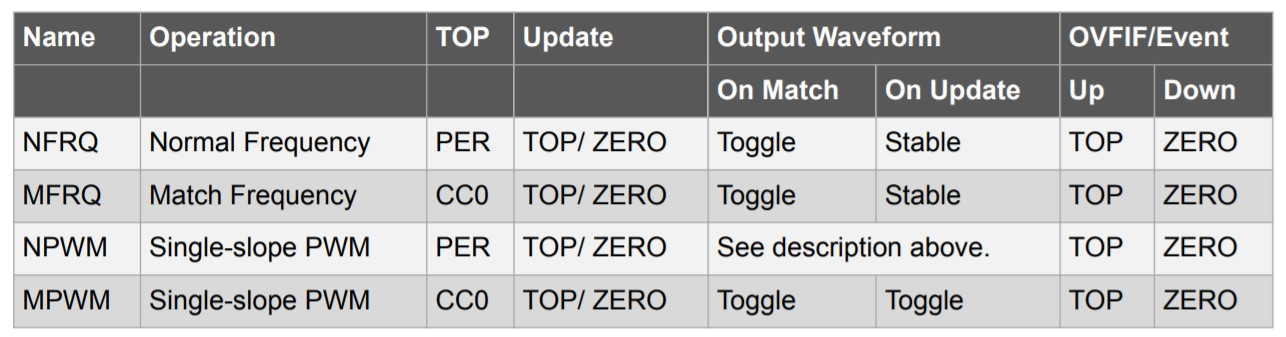
\includegraphics[width=12cm]{figure/mode Waveform.jpg}
\caption{Mode de fonctionnement en WAVEFORM pour les compteurs}
\label{pic1}
\end{figure}

Le mode Match Frequency Generation (MFRQ) est le plus adapté à l'application. En effet, la fréquence n'est fixée qu'avec un seul paramètre CC0. D'après la datasheet du SAMD21, le fonctionnement du mode MFRQ est le suivant. \\

\begin{figure}[H]
\centering
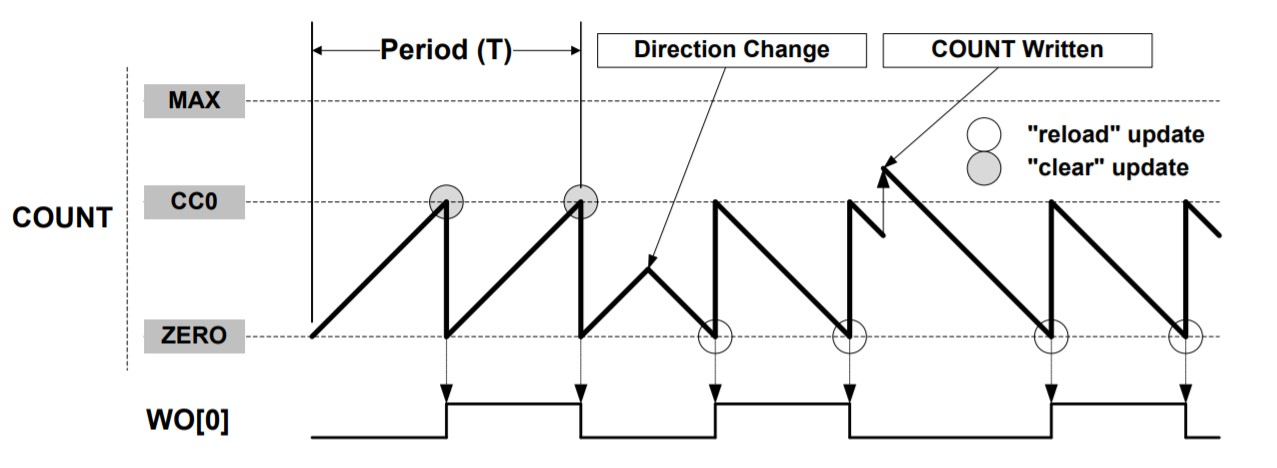
\includegraphics[width=12cm]{figure/Match Frequency Operation.jpg}
\caption{Fonctionnement timer configuré en MFRQ}
\label{pic2}
\end{figure}
La période T du signal est contrôlée par le registre CC0. Le signal de sortie est numérique, sa valeur se trouve dans WO[0]. A chaque fois que le compteur COUNT atteint la valeur du registre CC0.  Le signal de sortie WO[0] est permuté. La valeur MAX correspond à la résolution du compteur : ici 16 bits donc 65536 valeurs possibles. Il faudra être vigilent car la valeur du compteur vaut deux fois celle du signal de sortie.\\

\paragraph{Calculs pour une fréquence de 1kHz}
~~\\
Pour obtenir une fréquence de 1kHz il faut déterminer la valeur de CC0 comme expliqué précédemment. Pour faire cela il est primordial de bien comprendre son fonctionnement et les registres impliqués dans la configuration. La figure ci-dessous donne la fréquence de comptage. \\

\begin{figure}[htbp]
\centering
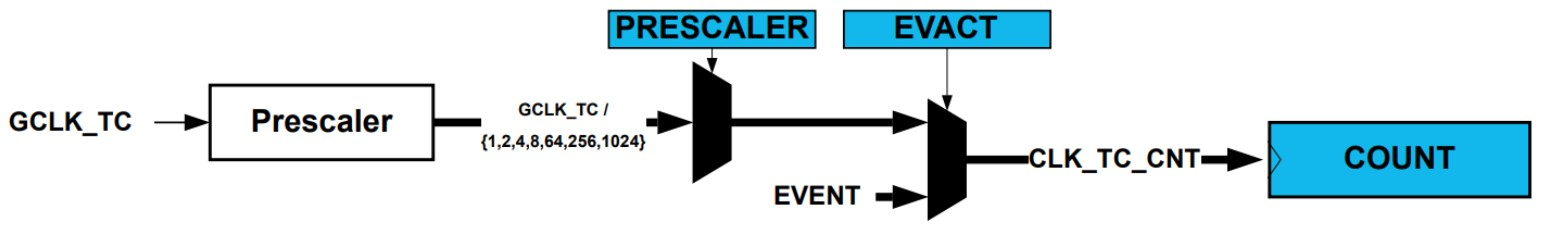
\includegraphics[width=12cm]{figure/prescaler.jpg}
\caption{Configuration du compteur TC}
\label{pic3}
\end{figure}

L'horloge count est fournie à partir de l’horloge GCLK\_TC (Generic clock for TC). Elle est l'horloge de référence pour les TC. Elle a une fréquence de 8MHz. Cette horloge peut être divisée en y appliquant un prescaler afin d’obtenir CLK\_TC\_CNT. N est une pré division de l’horloge du timer. Dans notre cas, le prescaler n’est pas appliqué et prendra la valeur N = 1. L'équation ci-dessous présente la fréquence à laquelle sera effectué le comptage. \\
\begin{equation}
	T_{GCLK\_TC} = N*T_{CLK\_TC\_CNT} = T_{CLK\_TC\_CNT}
\end{equation}

Donc
\begin{equation}
	f_{GCLK\_TC} = f_{CLK\_TC\_CNT}
\end{equation}
La fréquence souhaitée est établie à partir de l'équation suivante :
\begin{equation}
	f_{WO[0]} = \frac{f_{CLK\_TC\_CNT}}{2*(CC0+1)}
\end{equation}
On sait que $f_{GCLK\_TC}$ est égale à 8 MHz. Pour une fréquence $f_{WO[0]}$ de 1kHz, on obtient\\
\begin{equation}
	CC0 = \frac{f_{GCLK\_TC}}{2*f_{WO[0]}} - 1 = 3999
\end{equation}
La valeur chargée dans le registre CC0 sera donc 3999.
\subsection{Configuration TC6}
Configuration du TC6.


\newpage

\bibliography{lib}{}
\bibliographystyle{unsrt}

\end{document}

\begin{itemize}
	\renewcommand{\labelitemi}{--}
\end{itemize}